\chapter{Opis i ewaluacja wykonanej aplikacji}


Aplikacja, której implementacja jest opisana w tym rozdziale powstała w celu urozmaicenia zajęć prowadzonych na kierunku Automatyka i Robotyka. 
Ma ona za zadanie integrację symulatora jazdy i algorytmów wizyjnych implementowanych przez uczestników zajęć. 

\section{Przegląd dostępnych symulatorów}
\label{sec:ets2}

Na rynku jest dostępnych wiele symulatorów, które wpasowałyby się w ramy niniejszej pracy.
Pierwszym przykładem są gry z serii \textit{Grand Theft Auto} amerykańskiego studia Rockstar. 
Oferują one grafikę na wysokim poziomie, która wiernie oddaje rzeczywistość. 
Na ich niekorzyść przemawia fakt, że wspomniane gry nie zapewniają dobrego wsparcia dla programistów. 
Dodatkową wadą jest wysokie zużycie zasobów w stosunku do uzyskiwanej jakości obrazu (GTA V) lub niskie zużycie mocy obliczeniowej przy niskiej jakości grafiki (GTA: San Andreas).

Innym przykładem symulatorów są gry ze studia SCS Software. 
Obecnie w ofercie są dwie aplikacje: American Truck Simulator oraz Euro Truck Simulator 2. 
Oba symulatory są oparte na tym samym silniku graficznym i oferują podobne możliwości programistyczne. 
Aby zwiększyć różnorodność występujących elementów infrastruktury skupiono się na Euro Truck Simulator 2.
Za grą z czeskiego studia przemawiają następujące argumenty. 
Z uwagi na charakter niniejszej pracy, interesującymi elementami gry jest wysoka jakość grafiki, wiernie odwzorowująca otaczający świat, w tym zestaw znaków i linii drogowych charakterystycznych dla poszczególnych krajów Europy. 
Kolejnym elementem który przemawia za wyborem tego symulatora jest otwartość na wszelkie modyfikacje. 
Twórcy gry udostępnili API (ang. \textit{Application Programming Interface}), a także konsolę, za pomocą której można na bieżąco modyfikować parametry gry takie jak czas, prędkość gry lub pogodę.
Gra jest udostępniona na platformie Steam zarówno dla systemu Windows i Linux.

Fakt, że jest to symulator ciężarówki, a nie samochodu osobowego w żaden sposób nie wpływa na podejście do problemu systemów wizyjnych, ponieważ po pierwsze, istnieją aplikacje wspomagające kierowcę samochodu ciężarowego, po drugie jeden z widoków w grze jest umieszczony w miejscu, które znajduje się na wysokości lusterka samochodowego.


Wspomniana konsola dostępna w grze pozwala na natychmiastową zmianę warunków w symulatorze. 
Używając następujących komend można zmienić czas, pogodę oraz prędkość gry:

\begin{itemize}
\item g\_ set\_ weather x -- komenda zmieniająca pogodę. Gdy x jest równy 1, pogoda jest deszczowa, natomiast, gdy jest równy 0 pogoda jest słoneczna
\item g\_ set\_ time x -- komenda ustalająca godzinę w grze. W miejsce x należy podać godzinę w formacie hh,
\item warp x -- komenda zmieniająca prędkość gry. W miejsce x należy wpisać współczynnik. Liczba mniejsza od 1 zwolni grę, a większa przyspieszy.
\end{itemize}


\section{Wykorzystywane narzędzia programistyczne}


Do stworzenia aplikacji użyto następujących narzędzi/komponentów:
\begin{itemize}
\item Python 3.7 -- język programowania wysokiego poziomu ogólnego przeznaczenia,
\item gra Euro Truck Simulator 2,
\item SDK (ang. \textit{Software Development Kit}) udostępnione przez twórców gry,
\end{itemize}
a także bibliotek: 
\begin{itemize}
\item OpenCV 3.1.3 -- biblioteka zawierająca funkcje do cyfrowego przetwarzania obrazów,
\item threading -- biblioteka wspierająca programowanie wielowątkowe,
\item libWnck -- biblioteka zapewniająca komunikację ze środowiskiem graficznym (Window Navigator Construction Kit),
\item uinput -- biblioteka pozwalająca symulować kontroler do sterowania grą.
\end{itemize}

Aplikacja jest opracowana do działania na systemie Ubuntu 18.04 LTS wraz ze środowiskiem graficznym GNOME.

Jako, że opisywana aplikacja i symulator jest uruchamiany na jednym komputerze, należy zwrócić uwagę na wykorzystanie zasobów. 
W związku z tym wybranie niskich ustawień jakości grafiki pozwoli na przekazanie zasobów obliczeniowych do aplikacji.


\section{Architektura systemu}

Z uwagi na dydaktyczną wartość opisywanej aplikacji, ważnym elementem jest łatwość implementacji algorytmów analizy obrazu dla przyszłych użytkowników. 
Z tego powodu zdecydowano się na implementację wieloprocesową, której schemat jest widoczny na rysunku \ref{fig:arch}, w której jeden z procesów jest odpowiedzialny za analizę obrazu i wypracowanie sterowania, a pozostałe za poprawne przechwycenie obrazu z gry i zasymulowanie wypracowanego sterowania w grze. 

\begin{figure}
  \centering
  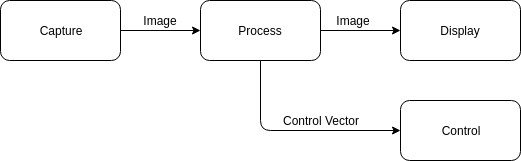
\includegraphics[width=13cm]{img/architektura.png}
  \caption{Schemat architektury aplikacji}
  \label{fig:arch}
\end{figure}

Poszczególne procesy są połączone kolejkami, za pomocą których odbywa się wymiana danych.
W przypadku opisywanej aplikacji w kolejkach umieszczane są obrazy wejściowe i wyjściowe z procesu $Process$, a także wektor sterowań do procesu $Control$. 
Szybkość działania aplikacji jest zależna od wielu czynników. 
Głównym elementem wpływającym na ten parametr, jest czas przetwarzania obrazu w bloku $Process$. 
W~zależności od liczby obrazów czekających na przetworzenie w kolejce zmieniany jest interwał pomiędzy poszczególnymi przechwyceniami obrazu w bloku $Capture$. 
Uniezależnienie przechwytywania obrazu od zapełnienia kolejki spowodowałoby szybkie jej przepełnienie i zamknięcie aplikacji przez system.  
Końcowe procesy tj. $Display$ i $Control$ nie wymagają wyzwalania w zależności od czasu przetwarzania obrazu, ponieważ wykonują się bardzo szybko (poniżej 10ms).

Używana biblioteka \textit{multiprocessing}\cite{S2} pozwala na tworzenie podprocesów. 
Istnieją dwie koncepcje zrównoleglania wykonywania operacji na CPU (ang. \textit{Central Processing Unit} -- centralna jednostka przetwarzająca). 
Przewaga wieloprocesowości nad wielowątkowością jest następująca. 
Każdy kolejny proces może być wykonywany na osobnym rdzeniu, a istniejące już są wykonywane równolegle. 
Przeciwnie jest w przypadku wielowątkowości --  wątki tworzone są w obrębie jednego procesora. Jednakże istotną wadą korzystania z procesów względem wątków jest fakt, ze ich tworzenie jest czasochłonne. 
W przypadku opisywanej aplikacji nie ma to jednak znaczenia, ponieważ grupa procesów jest tworzona tylko raz przy inicjalizacji.

\subsection{Przechwytywanie obrazu -- \textit{capture}}
\label{sec:mechanism}
Optymalnym rozwiązaniem byłoby przechwytywanie obrazu wprost z pamięci symulatora, lecz póki co API gry tego nie udostępnia. 
W procesie $Capture$ realizowane są dwa podzadania. 
Pierwsze polega na znalezieniu i aktywowaniu okna symulatora. 
Ma to na celu zapobiegnięcie przechwycenia obrazu, gdy okno gry jest przysłonięte przez inną aplikację lub zminimalizowane. 
Następnie, za pomocą biblioteki \texttt{libwnck} odczytywane są współrzędnych okna gry (współrzędne górnego rogu, szerokość i wysokość). 
Dopiero, gdy obraz znajdzie się w kolejce jest z niej pobierany przez kolejny proces i w postaci macierzy o wymiarach 1024x768x3 wysyłany do procesu przetwarzania i analizy obrazu. 
Jednorazowe przechwycenie okna zajmuje średnio około 10ms.

\subsection{Przetwarzanie i analiza obrazu -- \textit{process}}
Przetwarzanie i analiza obrazu odbywa się w bloku $Process$.
Jeśli kolejka wejściowa do procesu nie jest pusta, to obraz jest z niej pobierany, a następnie w zależności od wybranego algorytmu (np. detekcja linii, detekcja znaków) jest przetwarzany. 
Poszczególne opisy zaimplementowanych algorytmów znajdują się w rozdziale \ref{sec:implem}. 
Istotne jest, aby po skończeniu przetwarzania obrazu i wypracowaniu sterowania umieścić w kolejce rezultat z zaznaczonym wynikiem oraz wektorem sterowań w kolejce. 

\subsection{Symulacja kontrolera -- \textit{controller}}
Euro Truck Simulator 2 pozwala użytkownikowi na sterowanie ciężarówką za pomocą licznych kontrolerów. 
Może to być klawiatura, klawiatura w zestawie z myszką komputerową, kierownica lub gamepad. 
W systemach UNIX-owych każde urządzenie wejściowe podpięte do komputera jest widoczne jako plik w lokalizacji $\backslash dev\backslash input\backslash $. 
Urządzenia generują zdarzenia (ang. \textit{event}), które są przesyłane do korzystających z nich aplikacji.
Biblioteka $uinput$ pozwala na zasymulowanie dowolnego kontrolera i sterowanie nim programowo. 
Na potrzeby opisywanej aplikacji stworzono kontroler, która posiada trzy osie analogowe: kierownica, pedał gazu i pedał hamulca. 
Dodatkowo, w~celu umożliwienia programowego wpisywania komend do konsoli, kontroler posiada pełen zestaw klawiszy z układu QWERTY. 
Podczas uruchamiania aplikacji jest inicjalizowany kontrole tak, aby przed rozpoczęciem właściwej rozgrywki i przetwarzania obrazu gra wykryła poprawnie urządzenie do sterowania. 
Klasa $Control$ posiada metodę $emit$, która odpowiada za wygenerowanie zdarzenia z odpowiednimi wartościami sterowania. 
Podczas wykonywania tej metody jest sprawdzane czy okno z grą jest aktywne, ponieważ w przypadku symulowania sterowania przy nieaktywnym oknie, nie będzie ono poprawnie zinterpretowane przez grę. 

\subsection{Wyświetlanie rezultatów}

Wyświetlanie rezultatów jest opcjonalne. 
Jest realizowane w osobnym procesie ze względu na ustaloną architekturę systemu, która zakłada podział zadań. 
Oznacza to, że w bloku $Process$ jest dokonywana tylko analiza obrazu. 
Ma to na celu zminimalizowanie czasu potrzebnego na przetworzenie pojedynczej klatki. 
Wyświetlanie obrazu jest realizowane za pomocą funkcji biblioteki OpenCV $imshow()$.


\section{Opis implementacji algorytmów wizyjnych użytych w symulatorze}
\label{sec:implem}
W tym rozdziale zostaną opisane algorytmy służące do przetestowania działania aplikacji stworzonej w ramach pracy magisterskiej. 
Cele jakie są postawione przed systemem to: przetwarzanie obrazu w czasie rzeczywistym lub do niego zbliżonym oraz możliwość symulacji kontrolera i sterowanie wirtualnym pojazdem. 

\subsection{Algorytm detekcji linii}

W symulatorze Euro Truck Simulator 2 występuję typy dróg z każdego kraju Europy. 
Zaczynając od szerokich autostrad, poprzez drogi ekspresowe na wąskich i krętych drogach w Alpach kończąc. 
Zaimplementowany algorytm jest przeznaczony do detekcji linii na drogach, których krzywizna łuku nie jest duża. 
Przykładowy obraz wejściowy jest widoczny na rysunku \ref{fig:inputimg2}. 
Pierwszym krokiem jest konwersja przestrzeni barw z RGB do HSV. 
Wybranie składowej S jako obrazu poddawanego analizie (rys. \ref{fig:alg1_S}) pozwala uniezależnić się od pory dnia i pogody.

\begin{figure}
  \centering
  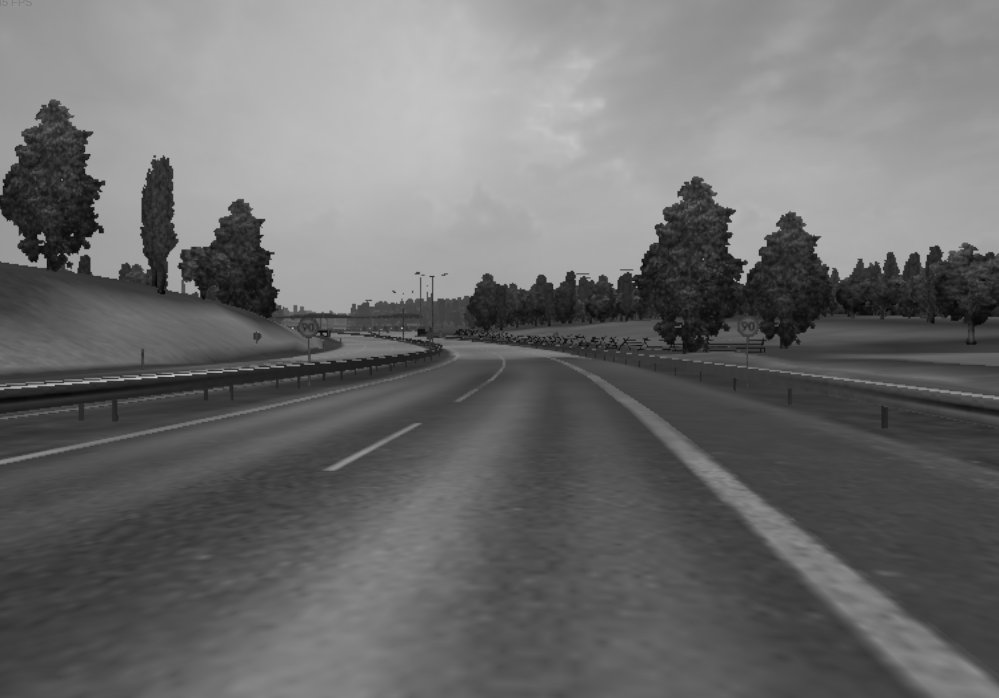
\includegraphics[width=7cm]{img/alg1_gray.jpg}
  \caption{Obraz wejściowy (składowa S)}
  \label{fig:alg1_S}
\end{figure}

\begin{figure}
  \centering
  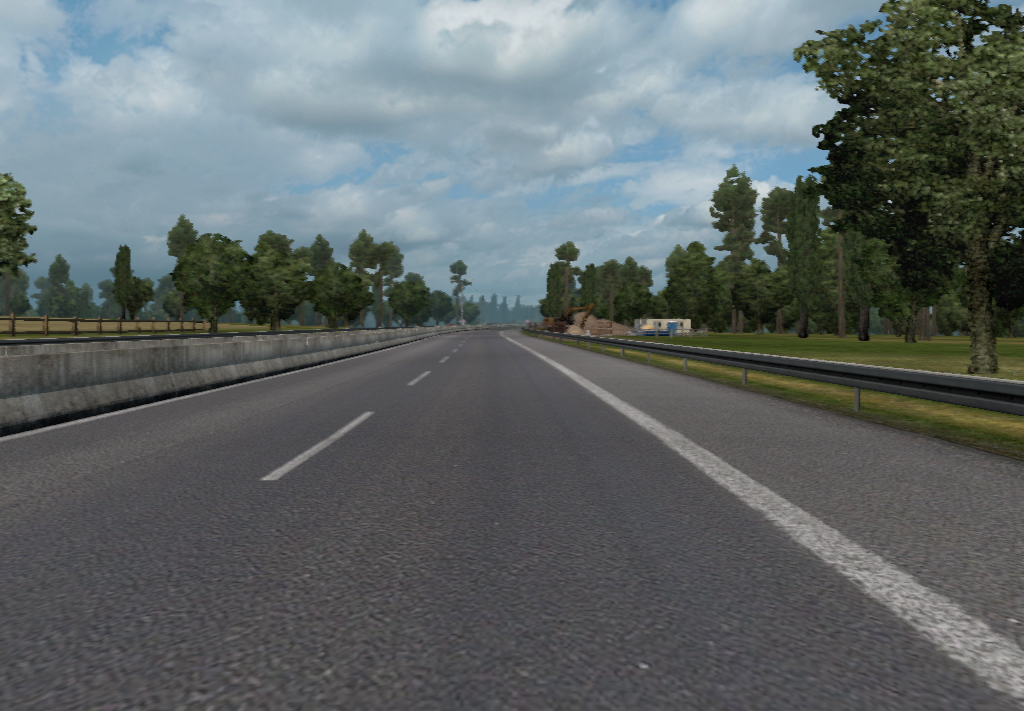
\includegraphics[width=7cm]{img/input.png}
  \caption{Przykładowy obraz wejściowy algorytmu detekcji pasa ruchu}
  \label{fig:inputimg2}
\end{figure}
  
Założenie, że obszar jezdni może znajdować się tylko na pewnym fragmencie obrazu pozwala zaoszczędzić czas obliczeń. 
Gdy znana jest orientacja kamery względem samochodu i podłoża można założyć że w górnej części obrazu i po bokach linie oddzielające pasy ruchu nie będą występować.
Po wybraniu ROI otrzymano obraz \ref{fig:alg1_roi}.


\begin{figure}[h]
	\centering
	\begin{subfigure}{0.35\textwidth}
		\centering
		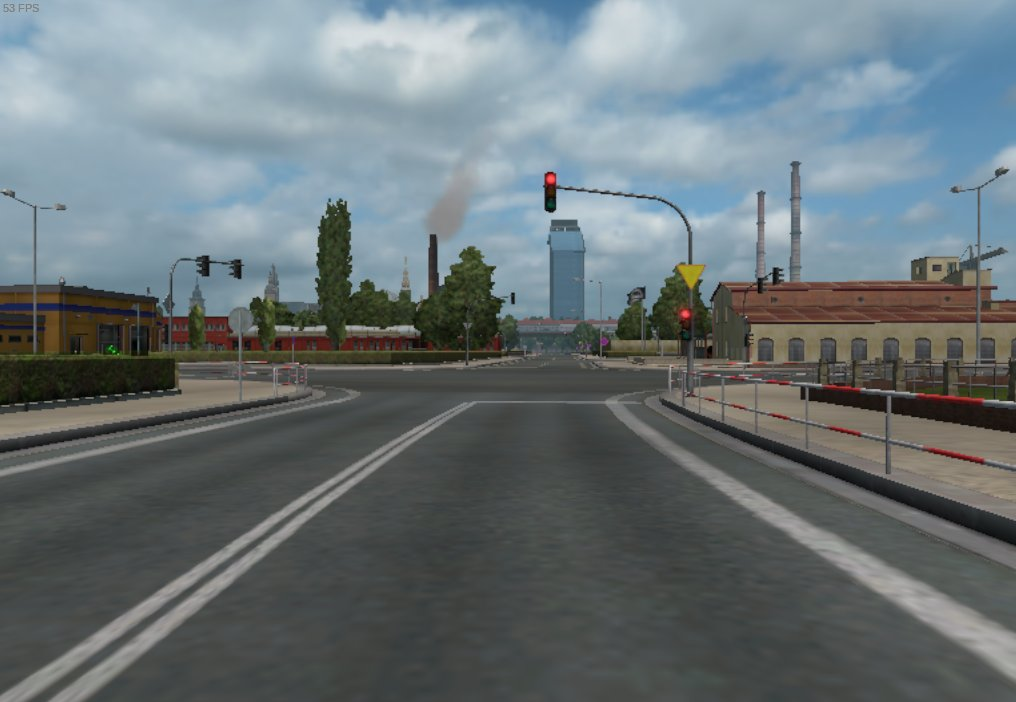
\includegraphics[width=6cm]{img/low_details.jpg}
		\subcaption{\label{fig:low_details}}
	\end{subfigure}
	\begin{subfigure}{0.35\textwidth}
		\centering
		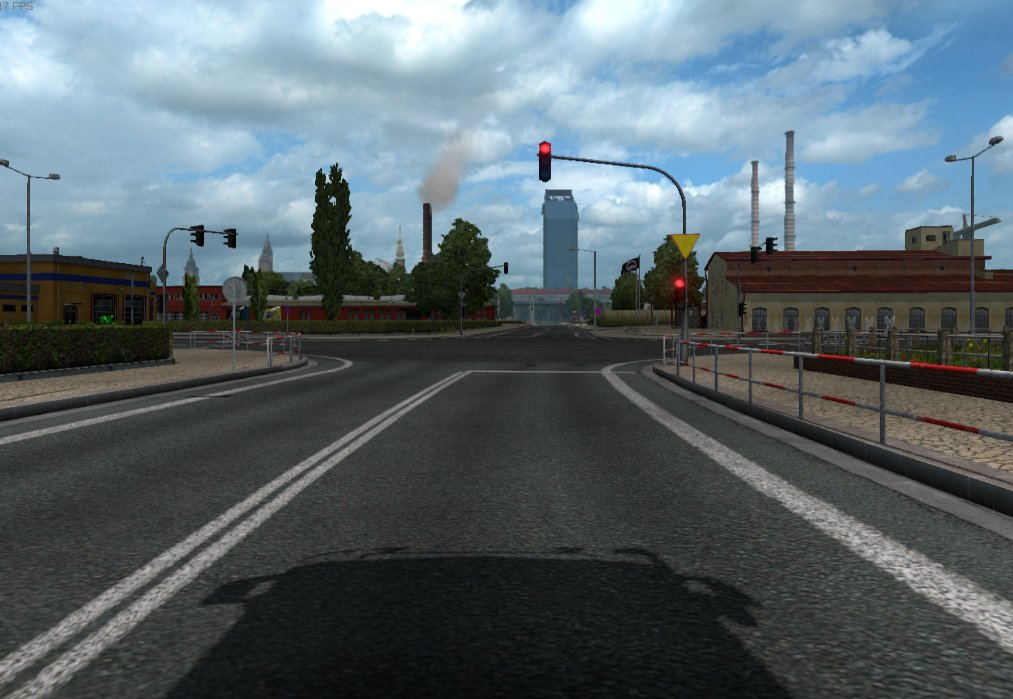
\includegraphics[width=6cm]{img/high_details.jpg}
		\subcaption{\label{fig:high_details}}
	\end{subfigure}
	
	\caption{\label{fig:details1}Porównanie ustawień niskiej \protect\subref{fig:low_details} i wysokiej \protect\subref{fig:high_details} jakości grafiki symulatora}
\end{figure}

Kolejnym krokiem jest wykrycie krawędzi z użyciem filtru Canny'ego. 
Progi zostały dobrane eksperymentalnie. 
Należy zwrócić uwagę, że gra pozwala na ustalenie jakości grafiki. 
W związku z tym, każdorazowo po zmianie ustawień należy dobrać współczynniki filtru na nowo. 
Wraz ze wzrostem jakości kształty renderowane w grze mają bardziej wyraźne krawędzie. 
Porównanie ustawień niskiej i wysokiej jakości grafiki w grze jest widoczne na rysunku \ref{fig:details1}. 

\begin{figure}
  \centering
  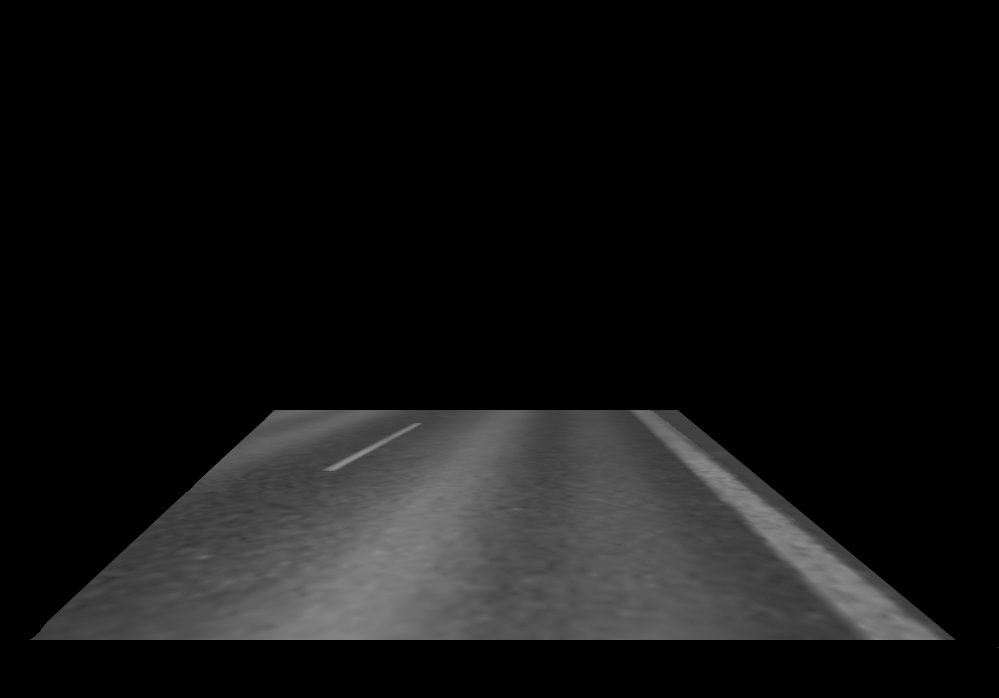
\includegraphics[width=13cm]{img/alg1_roi.jpg}
  \caption{Wyznaczone ROI, na którym można spodziewać się linii}
  \label{fig:alg1_roi}
\end{figure}

Na obrazie krawędzi, za pomocą transformaty Hougha wykonywana jest detekcji linii prostych. 
Linie fałszywe (linie nie będące liniami na jezdni) można odrzucić badając ich orientację. 
Właściwe linie będą pochylone pod odpowiednim kątem. 
Dla opisywanego przypadku zakresem kąta nachylenia linii jest $\theta < 1.3rad$ dla linii po lewej i $\theta > 2rad$ dla krawędzi prawej. 

W celu zmniejszenia czasu obliczeń i poprawienia sprawności algorytmu założono, że rezultatem powinna być linia dla każdej z krawędzi jezdni. 
Jeśli wykryto kilka linii, których parametry są zbliżone, dalszej analizie poddawana jest tylko jedna z nich, pierwsza, którą algorytm napotka na liście prostych. 
Pozostałe, których parametry są zbliżone są pomijane (rys. \ref{fig:alg1_res}).


Aby wygenerować sterowanie bada się punkt przecięcia wykrytych linii (biały okrąg na rys. \ref{fig:alg1_res}). 
Zakładając, że kamera jest ustawiona w osi ciężarówki można przyjąć, że każde odchylenie punktu przecięcia od punku równowagi znajdującego się w osi pojazdu powinno implikować ruch kierownicą.

\begin{figure}
  \centering
  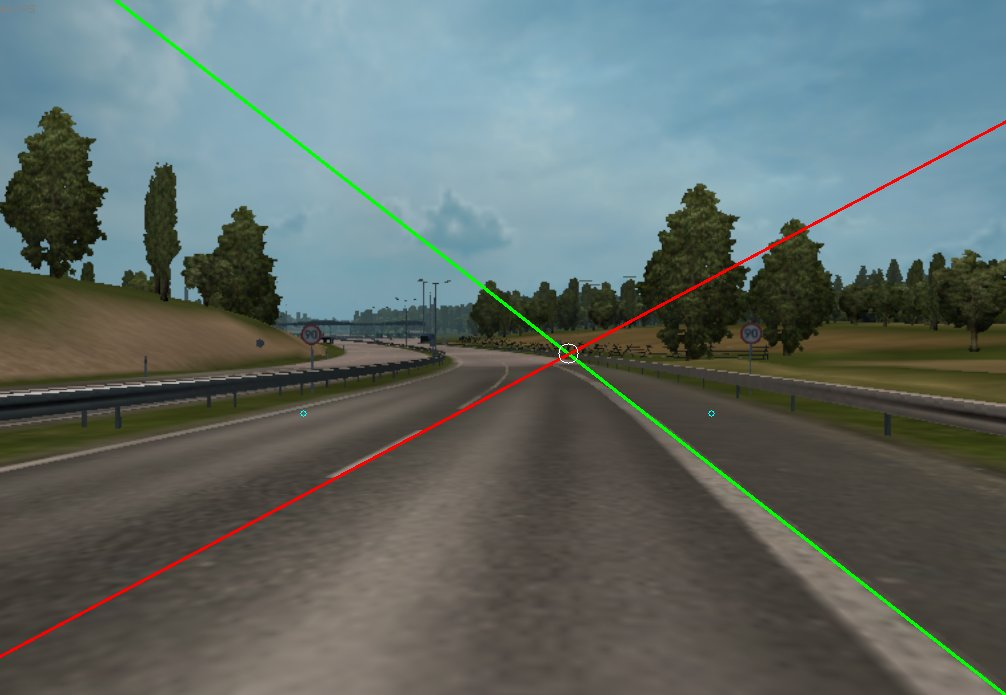
\includegraphics[width=13cm]{img/alg1_res.jpg}
  \caption{Rezultat działania algorytmu}
  \label{fig:alg1_res}
\end{figure}

Średni czas obliczeń potrzebny do przetworzenia jednej klatki wyniósł 59ms, co daje możliwość przetworzenia 17 klatek na sekundę. 
Jest to wydajność wystarczająca, aby zapewnić stabilność całości algorytmu, ponieważ ciężarówka była w stanie utrzymać się przy stałej prędkości na pasie ruchu długim na ok. 500m. 
Następnie algorytm traci stabilność. Jest częściowo spowodowane istnieniem pewnego opóźnienia pomiędzy odczytem obrazu, a momentem sterowania pojazdem.
%TODO a umie Pan wskazać przyczynę - w sensie czy to wina detekcji lini, czy czegoś innego OK

\subsection{Sytuacje potencjalnie problematyczne}

Jak wspomniano rozdziale \ref{sec:lane_detection} wymagane jest poprawne działanie algorytmu przy zmiennych warunkach oświetlenia i pogody. 
Symulator oferuje możliwość zmiany tych parametrów poprzez konsolę. 
Algorytm wykazał skuteczność zarówno przy zmianie godziny gry na późniejszą oraz dodaniu deszczu (rys. \ref{fig:alg1_late} i rys. \ref{fig:alg1_rain})

\begin{figure}
  \centering
  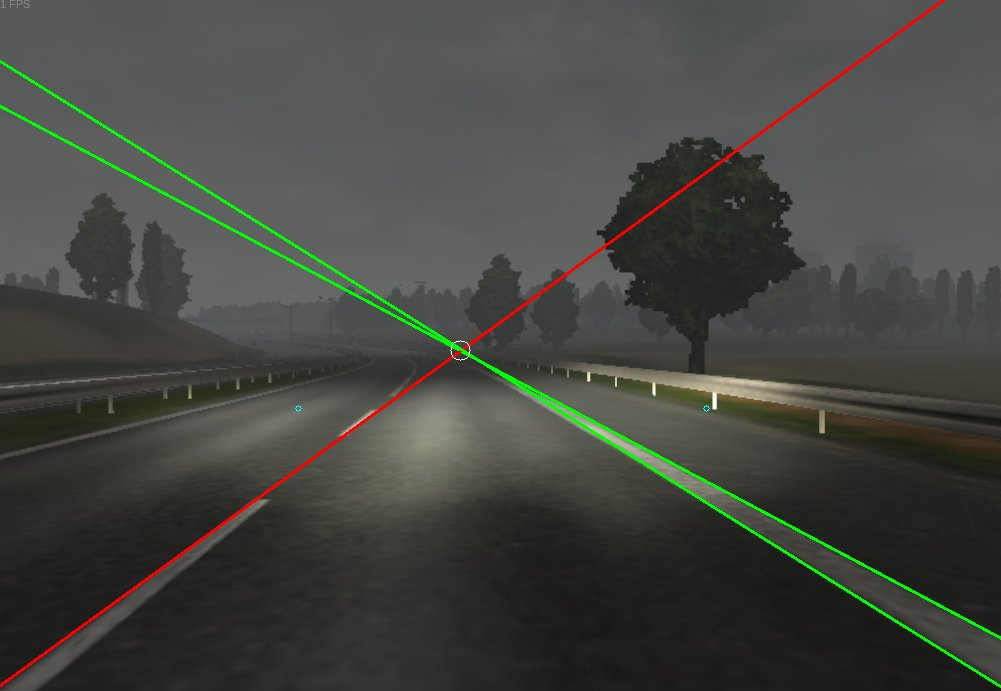
\includegraphics[width=9cm]{img/alg1_late.jpg}
  \caption{Działanie algorytmu podczas trudnych warunków oświetleniowych}
  \label{fig:alg1_late}
\end{figure}

\begin{figure}
  \centering
  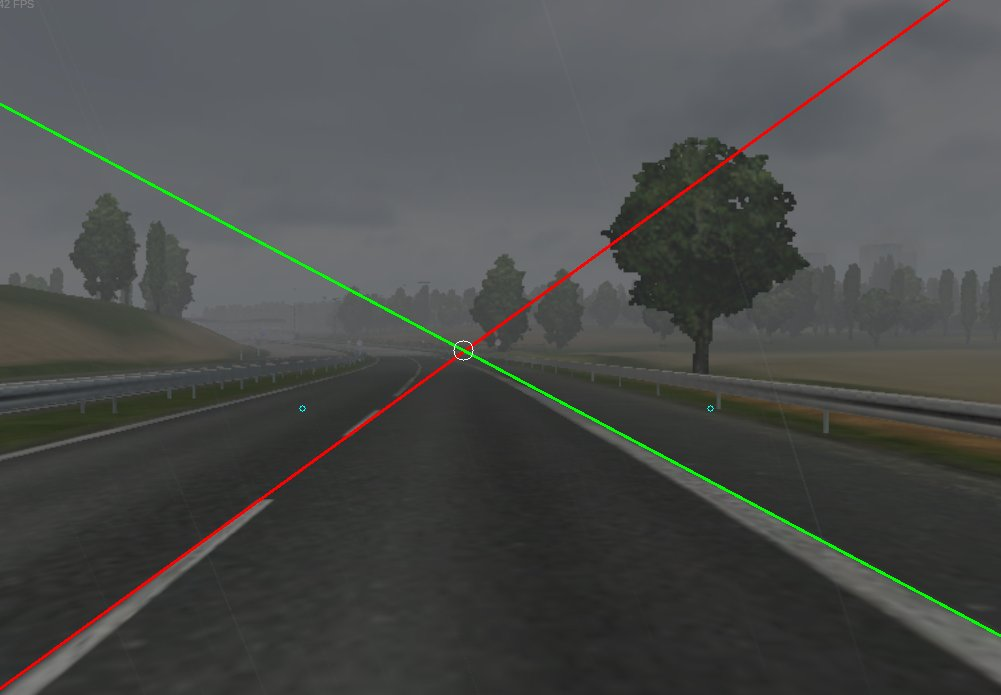
\includegraphics[width=9cm]{img/alg1_rain.jpg}
  \caption{Działanie algorytmu podczas deszczu}
  \label{fig:alg1_rain}
\end{figure}


\subsection{Algorytm detekcji czerwonych świateł sygnalizacji świetlnej} 

Kolejnym algorytmem testowym, który został zaimplementowany w ramach pracy jest uproszczona wersja algorytmu opisanego w rozdziale \ref{sec:tl}. 
Przykładowy obraz wejściowy znajduje się na rysunku \ref{fig:alg2_input}. 
Dają się tam zauważyć dwa sygnalizatory świetlne, a także kilka znaków drogowych. 
Sceneria została dobrana tak, aby jednocześnie sprawdzić odporność algorytmu na znaki zawierające czerwoną barwę.

Pierwszym krokiem opisywanej metody jest wyznaczenie kandydatów na elementy sygnalizatora świetlnego. 
Dobierając eksperymentalnie współczynniki progowania ustalono, że światło czerwone będzie spełniać poniższe warunki:
\begin{equation}
\label{eq:tl}
R>180 \wedge 0 \geq R<100 \wedge B < 120
\end{equation}

gdzie: $R, G, B$ oznaczają wartości składowych w przestrzeni RGB.

Aby zapewnić, że inne obiekty spełniające warunek \ref{eq:tl}, które nie są elementami sygnalizatora świetlnego, nie zostaną błędnie wykryte, wykonano operację progowania, a następnie erozji i dylatacji zwaną również otwarciem morfologicznym. %TODO czegoś tu brakuje - nadal czegość brakuje !!! OK
Otrzymany obraz poddawany jest indeksacji. 
Iterując po każdym z wyznaczonych elementów można sprawdzić jego powierzchnię i proporcje. 
Muszą one spełniać określone warunki, aby zostać uznane za światło sygnalizatora drogowego: powierzchnia powinna być większa niż 20 pikseli, a także stosunek szerokości do wysokości powinien zawierać się w przedziale $[0.75, 1.25]$.

Aby zmodyfikować algorytm tak, by wykrywał światło zielone lub pomarańczowe należy zmienić wartości progów w warunku \ref{eq:tl}. 
Do indeksacji kandydatów wykorzystano funkcję biblioteki OpenCV $connectedComponentsWithStats()$, która zwraca listę obiektów wraz z ich statystykami.

\begin{figure}
  \centering
  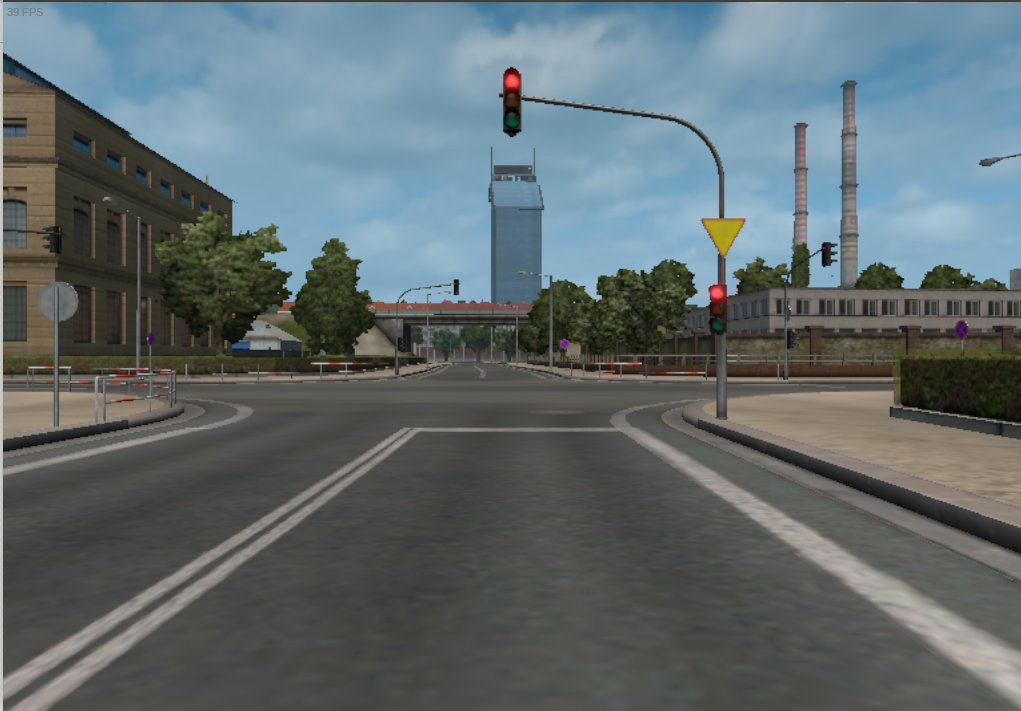
\includegraphics[width=9cm]{img/alg2_input.jpg}
  \caption{Przykładowy obraz wejściowy algorytmu}
  \label{fig:alg2_input}
\end{figure}

\begin{figure}
  \centering
  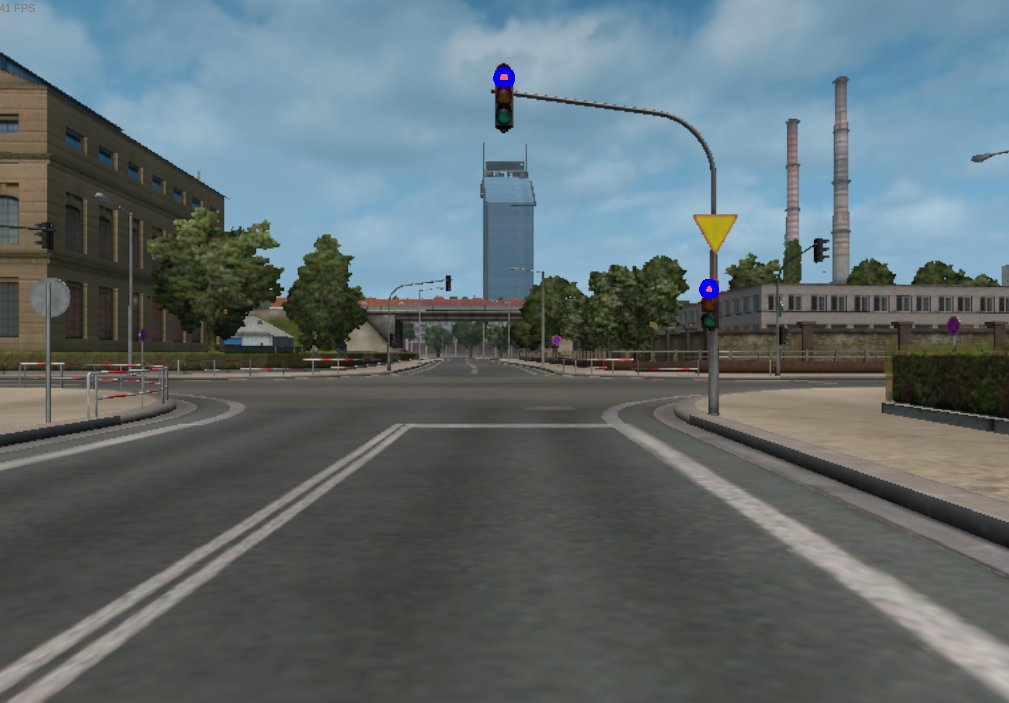
\includegraphics[width=9cm]{img/alg2_res.jpg}
  \caption{Wykryte dwa światła czerwone}
  \label{fig:alg2_res}
\end{figure}

\subsection{Sytuacje potencjalnie problematyczne}
Jak w przypadku każdego z omawianych algorytmów problemem jest zmiana warunków oświetleniowych oraz pogodowych. 
Nie można jak w przypadku algorytmu detekcji pasa ruchu uniezależnić się od zmian oświetlenia poprzez zastosowanie konwersji do przestrzeni HSV, ponieważ istotną rolę odgrywa tu barwa. %TODO no teoretycznie można - H... nie próbował Pan pewnie. - oczywiście, że teoretycznie można, ale robić progowanie w przestrzeni HSV, gdy interesuje nas barwa chyba mija się z celem, albo będzie przynajmniej równoważne z robieniem tego w RGB. TK: No nie, tzn. powinno być lepiej, ale to nie ten czas i miejsce.
Z uwagi na to, że sygnalizatory emitują światło, w czasie warunków słabej widoczności i deszczu algorytm poprawnie wykrywał czerwone światło (rys. \ref{fig:alg2_rain} i rys. \ref{fig:alg2_late}).

\begin{figure}
  \centering
  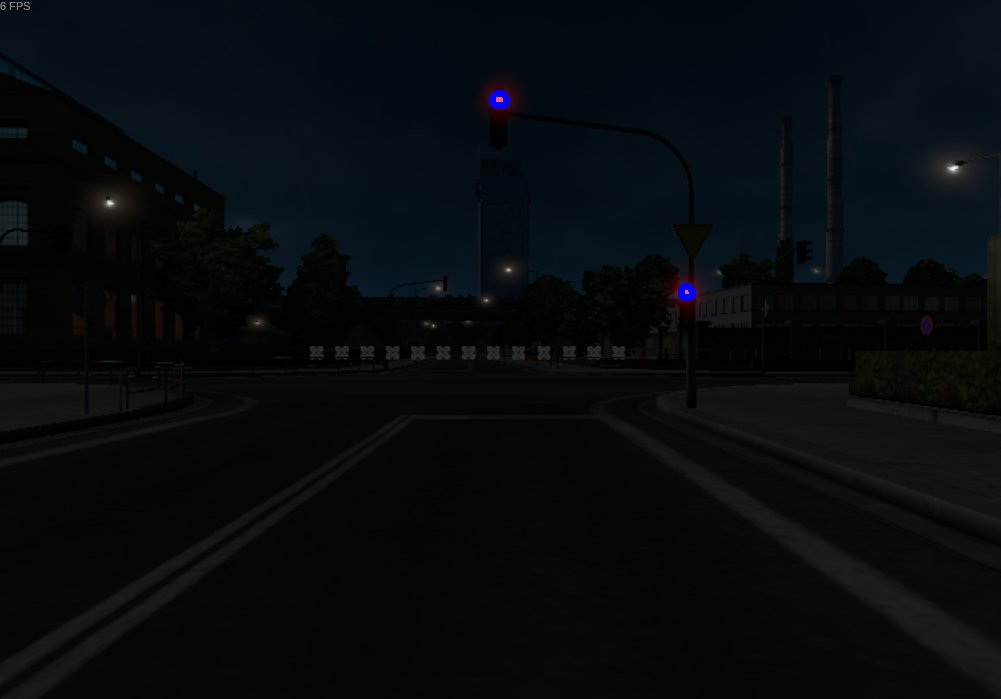
\includegraphics[width=9cm]{img/alg2_late.jpg}
  \caption{Wykryta sygnalizacja świetlna w warunkach słabego oświetlenia}
  \label{fig:alg2_late}
\end{figure}

\begin{figure}
  \centering
  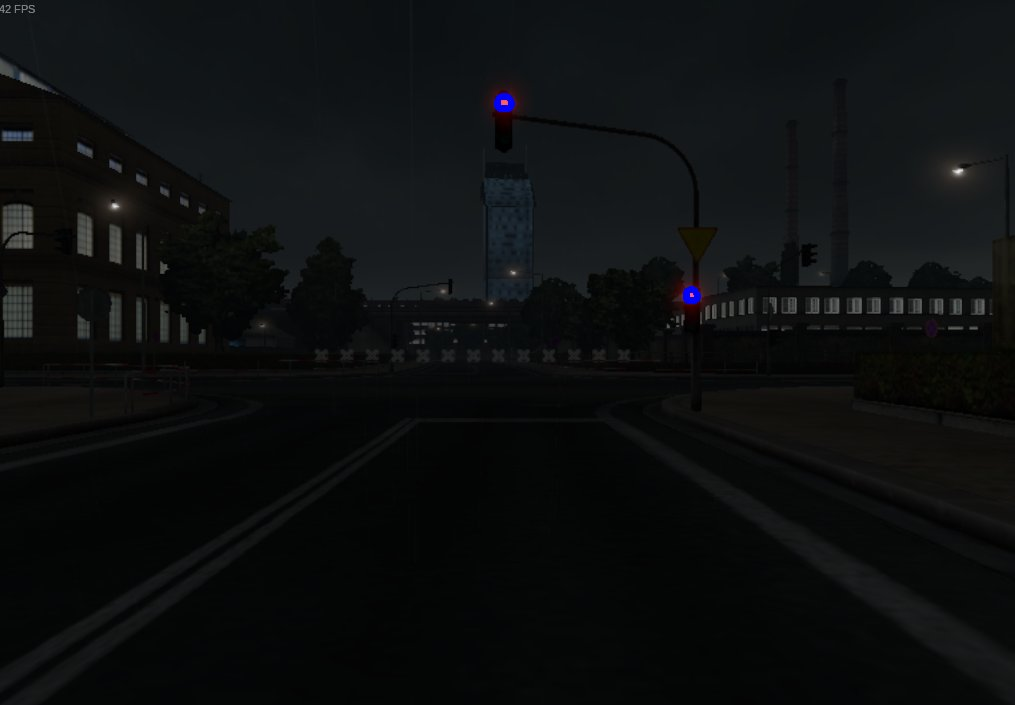
\includegraphics[width=9cm]{img/alg2_rain.jpg}
  \caption{Wykryta sygnalizacja świetlna podczas deszczu} 
  \label{fig:alg2_rain}
\end{figure}

%TODO a z tym było jakieś sterowanie związane ? jest powiedziane dalej - że do tego byłby potrzebny jakiś supervisor do tych wszystkich systemów, dane o lokalizacji, układzie drogi itp. Chyba żeby robić scenariusz, że jedziemy wprost na sygnalizator z czerwonym i trzeba się zatrzymać, to jest jak najbardziej do realizacji.

\subsection{Detekcja samochodu poprzedzającego}
Ostatnim algorytmem, który został zaimplementowany w ramach tej pracy była detekcja samochodów poprzedzających na drodze z użyciem detektora symetrii. 
Implementacja bazuje na algorytmie opisanym w rozdziale \ref{sec:car_general}. 

\begin{figure}
  \centering
  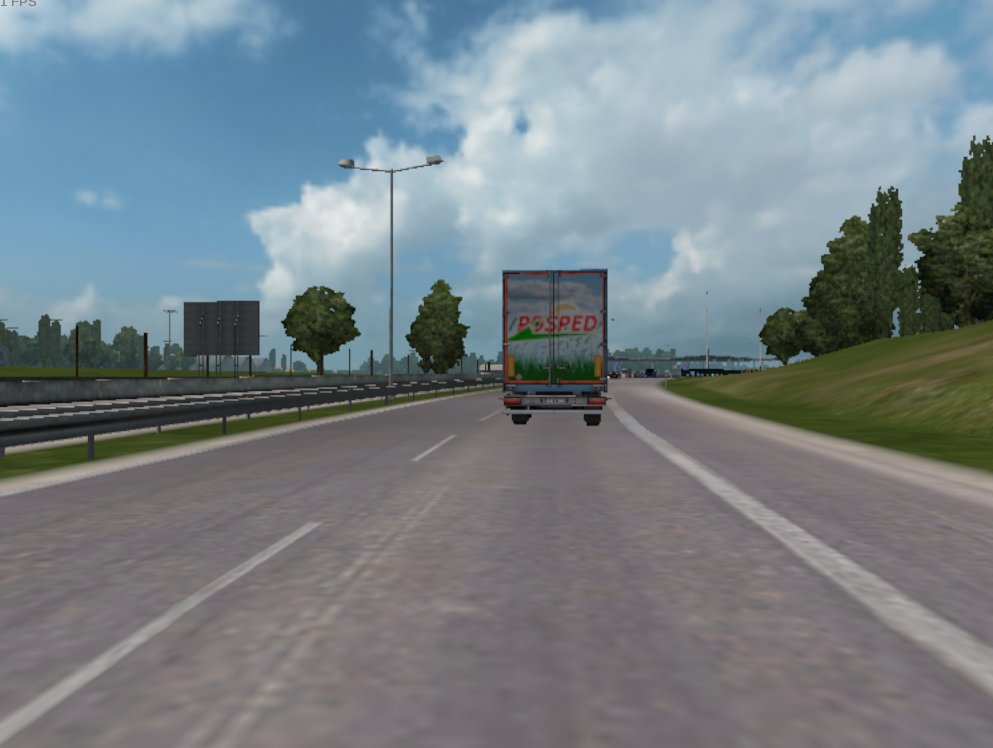
\includegraphics[width=9cm]{img/alg3_input.jpg}
  \caption{Przykładowy obraz wejściowy algorytmu detekcji samochodu poprzedzającego}
  \label{fig:alg3_input}
\end{figure}

Zaimplementowany algorytm jako argumenty przyjmuje obrazy w skali szarości. 
Przykładowy obraz wejściowy jest pokazany na rysunku \ref{fig:alg3_input}. 
Daje się na nim zauważyć ciężarówkę poprzedzającą samochód. 
Celem działania algorytmu jest poprawne wykrycie symetrii na tyle naczepy samochodu.

\begin{figure}
  \centering
  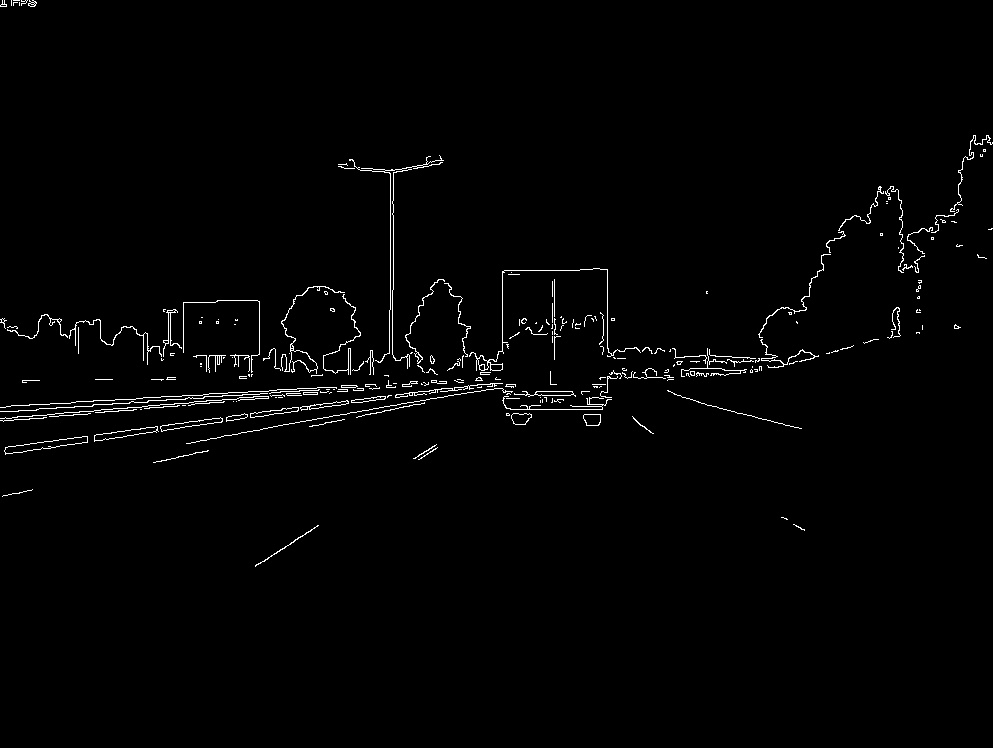
\includegraphics[width=9cm]{img/alg3_canny.jpg}
  \caption{Obraz wejściowy po detekcji krawędzi. Widoczna symetria w układzie krawędzi poprzedzającej naczepy}
  \label{fig:alg3_canny}
\end{figure}

Pierwszym krokiem jest filtracja z użyciem filtru Canny'ego. 
Progi filtru są dobierane eksperymentalnie każdorazowo po zmianie ustawień graficznych symulatora. 
Efekt filtracji jest widoczny na rysunku \ref{fig:alg3_canny}.

Następnie dla wybranych linii  sprawdzana jest symetria obrazów w sposób opisany w rozdziale \ref{sec:car_general}.
Na każdej z linii wyznaczane są maksima, które wskazują na istnienie osi symetrii. 
Rezultaty detekcji są przedstawione na rysunkach \ref{fig:alg3_res1} i \ref{fig:alg3_res2}. 
Daje się zauważyć znaczna liczba detekcji fałszywych. 
Prawdopodobnie wynika to między innymi z faktu, że w symulatorze obiekty infrastruktury mają bardziej równomierny i symetryczny kształt.


\begin{figure}
  \centering
  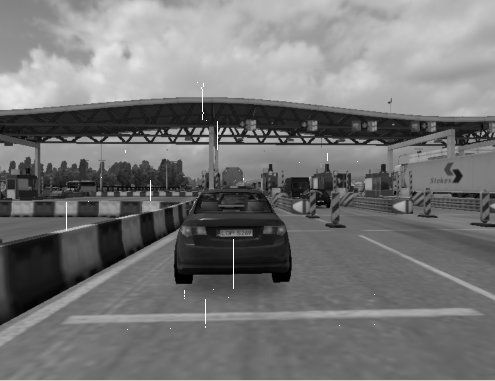
\includegraphics[width=9cm]{img/alg3_res.jpg}
  \caption{Rezultat detekcji samochodu osobowego. Widoczne liczne fałszywe detekcje.}
  \label{fig:alg3_res1}
\end{figure}

\begin{figure}
  \centering
  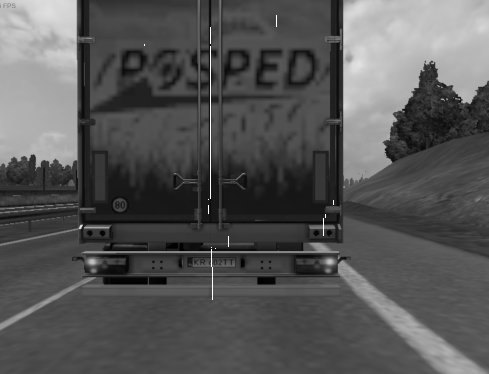
\includegraphics[width=9cm]{img/alg3_res2.jpg}
  \caption{Poprawna detekcja naczepy samochodu ciężarowego}
  \label{fig:alg3_res2}
\end{figure}

Sprawdzono również zachowanie algorytmu w trudnych warunkach pogodowych i przy słabym oświetleniu. 
Samochód korzysta ze świateł mijania, więc najbliższe otoczenie jest dobrze widoczne (rys. \ref{fig:alg3_rain_late}. 
W tym przypadku również pojawiają się fałszywe detekcje.

\begin{figure}
  \centering
  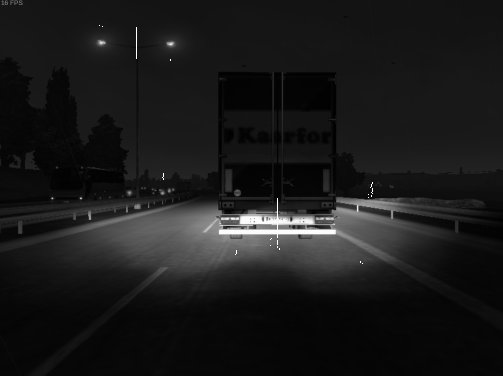
\includegraphics[width=9cm]{img/alg3_res3.jpg}
  \caption{Poprawna detekcja naczepy samochodu ciężarowego w trudnych warunkach oświetleniowych i pogodowych}
  \label{fig:alg3_rain_late}
\end{figure}

Obliczanie wskaźnika symetrii jest operacją bardzo czasochłonną. 
Średni czas przetworzenia jednej ramki to 5.45 sekundy. 
Oprócz dużej liczby obliczeń może to być spowodowane mało wydajną implementacją w Pythonie. 
Implementacja w języku C++ prawdopodobnie przyniosłaby lepsze efekty.

\section{Badania wydajności aplikacji}

Istotnym parametrem jest wydajność całej aplikacji. 
Powinna ona działać bez widocznych opóźnień, to znaczy, że po przechwyceniu obrazu z symulatora w możliwie najkrótszym czasie powinno zostać wygenerowane sterowanie. 
Jest to zapewnione poprzez mechanizm opisany w rozdziale \ref{sec:mechanism}. 
Eksperymentalnie sprawdzono, że liczba elementów w kolejkach, zwłaszcza w kolejce pomiędzy modułem $Capture$, a $Process$ nie powinna przekraczać 50. 
Powyżej tej wartości daje się zauważyć widoczne opóźnienie reakcji systemu sterującego samochodem. 
Na wykresie przedstawiono rozmiar kolejki w kolejnych iteracjach programu podczas działania systemu wizyjnego odpowiedzialnego za detekcję czerwonego światła.

\begin{figure}
  \centering
  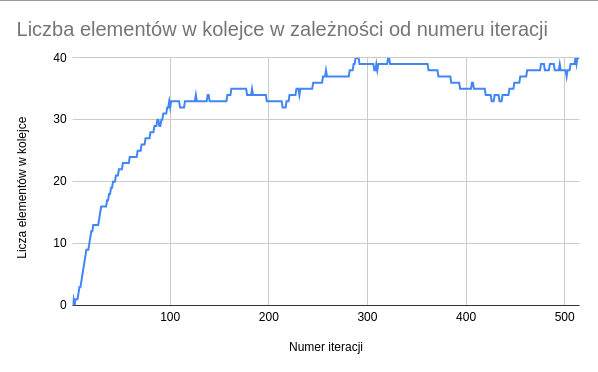
\includegraphics[width=9cm]{img/queue_stats.png}
  \caption{Rozmiar kolejki w trakcie działania programu}
  \label{fig:queue_stats}
\end{figure}

W trakcie implementacji kolejnych systemów wizyjnych używanych w pojazdach autonomicznych należy zwrócić uwagę na optymalizację kodu. 
Nie powinno się tworzyć wielu kopii obrazu w pamięci, a także, z uwagi na asynchroniczny charakter aplikacji,  używać komend typu $wait()$. 
Ważnym aspektem, który znacząco poprawił wydajność całości systemu było zastosowanie wektoryzacji, czyli wbudowanej w język programowania metody operowania na macierzach. 
W przypadku, gdy algorytm ze względu na swoją złożoność wykonywałby się zbyt długo, należy użyć komendy w konsoli symulatora udostępnionej przez twórców, która zmieni prędkość gry -- $warp x$, gdzie $x$ oznacza prędkość (1 -- standardowa prędkość rozgrywki).

Jak wspominano w poprzednich rozdziałach istotne jest zachowanie balansu w wykorzystaniu zasobów pomiędzy symulatorem Euro Truck Simulator 2, a aplikacją opisaną w tej pracy. 
Zbyt wysokie ustawienia jakości grafiki mogą spowodować, że przetwarzanie przechwyconych ramek nie będzie wykonywane wystarczająco szybko. 
Z kolei w przypadku najniższych ustawień jakości grafiki zasoby będą wystarczające do działania aplikacji, lecz może zdarzyć się sytuacja, że jakość grafiki będzie na poziomie, który nie pozwoli na poprawną detekcję znaków lub świateł drogowych (wysokie rozmycie grafiki).

\section{Ewaluacja systemu}

Celem pracy było stworzenie aplikacji, która będzie pozwalała w przyjazny użytkownikowi sposób na implementację i testowanie algorytmów wizyjnych stosowanych w pojazdach autonomicznych -- przykładowo w ramach przedmiotu Systemy i Algorytmy Percepcji Pojazdów Autonomicznych prowadzonego na II stopniu studiów stacjonarnych na kierunku Automatyka i Robotyka . 
Przykładowe algorytmy zaimplementowane w ramach tej pracy dowodzą, że jest to możliwe. 
Korzystanie z aplikacji w ramach zajęć jest zamienną formą w stosunku do korzystania ze zbiorów zdjęć np. KITTI \cite{W6}. 
Nie jest możliwe wygenerowanie wyników referencyjnych ($ground truth$), aczkolwiek inną formą sprawdzenia czy dany algorytm działa poprawnie jest weryfikacja poprzez zachowanie ciężarówki w symulowanym świecie. 
Opcjonalne jest generowanie sterowania na podstawie wyników z algorytmów wizyjnych. 
Końcowy użytkownik może tradycyjnie za pomocą klawiatury lub myszki sterować pojazdem i na bieżąco badać rezultaty osiągane przez algorytm.

Opracowana aplikacja zakłada, że sterowanie generowane jest na podstawie obrazu z bieżącej chwili. Nie ma żadnego elementu nadrzędnego, który koordynowałby działanie zaimplementowanych systemów.

W przypadku bardziej złożonych algorytmów pojawia się problem z wydajnością. 
Aplikacja nie jest w stanie na bieżąco analizować obrazu i generować sterowania. 
Zdarzają się sytuacje, że sterowanie jest generowane dla obrazu sprzed kilkuset milisekund, co wprowadza oscylacje pojazdu w przypadku algorytmu detekcji linii.
Proponowanym rozwiązaniem jest wprowadzenie pomijania kilku klatek przechwyconych z symulatora lub większy interwał czasowy pomiędzy klatkami.

Kolejnym etapem rozwoju projektu byłoby stworzenie prostego instalatora, który pobierze i zainstaluje wszystkie potrzebne biblioteki, a także skompiluje zmodyfikowane SDK udostępnione przez twórców. 
Możliwa jest także dalsza edycja SDK, poprzez umożliwienie odczytu pozostałych zmiennych gry oprócz aktualnej prędkości i stanu pauzy. 
Pełna lista parametrów jest dostępna w \cite{S3}. 
Elementem rozbudowującym aplikację byłoby także generowanie danych radarowych lub lidarowych na podstawie otoczenia samochodu w symulatorze. 
Póki co twórcy gry nie udostępniają takiej możliwości przez SDK.



\chapter{Podsumowanie}

W ramach pracy podjęto temat możliwości wykorzystania symulacji/gry do tworzenia i~ewaluacji algorytmów stosowanych w~zaawansowanych systemach wspomagania kierowym i pojazdach autonomicznych.
W części teoretycznej zawarto szerokie porównanie algorytmów wizyjnych stosowanych w pojazdach autonomicznych. 
Dokonano porównania dwóch wersji działających w tradycyjnym podejściu, a także zweryfikowano działanie metod opartych o głębokie uczenie. 

W części opisowej projektu najpierw scharakteryzowano, a następnie uzasadniono wybór wieloprocesowej architektury systemu.
Kolejno przetestowano działanie wybranych algorytmów wizyjnych z użyciem aplikacji. Jeden z nich (detekcja pasa ruchu) był sprawdzany w sytuacji ruchu symulowanego pojazdu i w ograniczonym zakresie był w stanie poprawnie kierować samochodem. Pozostałe algorytmy były testowane w warunkach statycznych, bez generowania sterowania.

%TODO kilka zdań o praktyce - tj. o aplikacji OK

Zdaniem autora przygotowana aplikacja nadaje się do użycia w ramach zajęć dydaktycznych.
Pozwala w łatwy sposób modyfikować parametry obrazu takie jak natężenie światła, pogodę oraz liczbę otaczających pojazdów. 

Znaczącą przewagą systemu nad analizą pojedynczych zdjęć jest możliwość przetestowania algorytmów w sytuacjach dynamicznych. 
Zaimplementowana możliwość sterowania samochodem w symulatorze z pewnością pozwoli na rozbudowanie i testowanie powstających algorytmów wizyjnych. 
Symulator pozwala na implementację funkcjonalności analogicznych z rzeczywistymi systemami w pojazdach autonomicznych.

Końcowym elementem pracy jest dodatek w postaci instrukcji (\ref{cha:appendix}) do ćwiczeń laboratoryjnych oraz pomoc w konfiguracji środowiska. 
Po wykonaniu instrukcji użytkownik może przystąpić do implementacji systemu wizyjnego.
%TODO ref do tego dodatku OK

